\documentclass[margin=1pt]{standalone}
\usepackage{color,xcolor}
\usepackage{makecell}
\usepackage{tikz-qtree, tikz}
\usetikzlibrary{arrows.meta,bending}
\usetikzlibrary{calc,trees,positioning,arrows,chains,shapes, shapes.geometric,%
    decorations.pathreplacing,decorations.pathmorphing,decorations.markings,shapes,%
    matrix,shapes.symbols,positioning,angles,quotes,patterns}
\usepackage[utf8]{inputenc}

%See https://tex.stackexchange.com/a/29367/1952
\makeatletter
\tikzset{% customization of pattern
        hatch distance/.store in=\hatchdistance,
        hatch distance=5pt,
        hatch thickness/.store in=\hatchthickness,
        hatch thickness=5pt
        }
\pgfdeclarepatternformonly[\hatchdistance,\hatchthickness]{north east hatch}% name
    {\pgfqpoint{-1pt}{-1pt}}% below left
    {\pgfqpoint{\hatchdistance}{\hatchdistance}}% above right
    {\pgfpoint{\hatchdistance-1pt}{\hatchdistance-1pt}}%
    {
        \pgfsetcolor{\tikz@pattern@color}
        \pgfsetlinewidth{\hatchthickness}
        \pgfpathmoveto{\pgfqpoint{0pt}{0pt}}
        \pgfpathlineto{\pgfqpoint{\hatchdistance}{\hatchdistance}}
        \pgfusepath{stroke}
    }
\makeatother

% Drawing spirals
\makeatletter
\newif\ifspiral@is@clockwise
  \pgfkeys{
    spiral/.is family,
    spiral,
    start angle/.initial=0,
    end angle/.initial=0,
    start radius/.initial=0,
    end radius/.initial=1,
    revolutions/.initial=2,
    name/.initial=,
    center/.initial={(0,0)},
    sample rate/.initial =5,
    clockwise spiral/.is if=spiral@is@clockwise,
    clockwise spiral/.default=false,
    clockwise/.style={clockwise spiral=true},
    default spiral/.style={start angle=0,end angle=0, start radius=0, end radius=1, revolutions=2, name=, center={(0,0)}, sample rate=5, clockwise spiral=false}
  }
  \newcommand\spiral[2][]{
    \pgfkeys{spiral, default spiral,#2,
      start angle/.get=\spiral@start@angle,
      end angle/.get=\spiral@end@angle,
      start radius/.get=\spiral@start@radius,
      end radius/.get=\spiral@end@radius,
      revolutions/.get=\spiral@revolutions,
      name/.get=\spiral@name,
      sample rate/.get=\spiral@sample@rate,
      center/.get=\spiral@center
      }
  \def\spiral@start@name{}
  \def\spiral@end@name{}
  \ifspiral@is@clockwise
        \renewcommand*{\spiral@start@angle}{\pgfkeysvalueof{/spiral/end angle}}
        \renewcommand*{\spiral@end@angle}{\pgfkeysvalueof{/spiral/start angle}}
        \renewcommand*{\spiral@start@radius}{\pgfkeysvalueof{/spiral/end radius}}
        \renewcommand*{\spiral@end@radius}{\pgfkeysvalueof{/spiral/start radius}}
        \if\relax\detokenize{\spiral@name}\relax
        \else
          \renewcommand*{\spiral@start@name}{\spiral@name end}
          \renewcommand*{\spiral@end@name}{\spiral@name start}
        \fi
    \else
        \if\relax\detokenize{\spiral@name}\relax
        \else
          \renewcommand*{\spiral@start@name}{\spiral@name start}
          \renewcommand*{\spiral@end@name}{\spiral@name end}
        \fi
  \fi
  \pgfmathsetmacro{\spiral@domain}{\spiral@end@angle+\spiral@revolutions*360}
  \pgfmathsetmacro{\spiral@growth}{180*(\spiral@end@radius-\spiral@start@radius)/(pi*(\spiral@domain-\spiral@start@angle))}
  \draw [#1,
         shift={\spiral@center},
         domain=\spiral@start@angle*pi/180:\spiral@domain*pi/180,
         variable=\t,
         smooth,
         samples=int(\spiral@domain/\spiral@sample@rate)] node[coordinate,shift={(\spiral@start@angle:\spiral@start@radius)}](\spiral@start@name){} plot ({\t r}: {\spiral@start@radius+\spiral@growth*\t-\spiral@growth*\spiral@start@angle*pi/180}) node[coordinate](\spiral@end@name){}
  }
\makeatother

\definecolor{myblue}{HTML}{0072BD}
\definecolor{mygreen}{HTML}{258F1B}
\definecolor{myred}{HTML}{C4000C}

\newcommand{\Ms}{\ensuremath{M_\mathrm{s}}} % Martensite start Temperature
\newcommand{\Mf}{\ensuremath{M_\mathrm{f}}} % Martensite finish Temperature
\newcommand{\As}{\ensuremath{A_\mathrm{s}}} % Austenite start Temperature
\newcommand{\Af}{\ensuremath{A_\mathrm{f}}} % Austenite finish Temperature

\tikzset{
  pivot_node/.style = {
    inner sep=0pt, minimum width=1.18cm,minimum height=2.15cm,
    path picture={
    % screen (with border)
        \node (piv) {};
        % \spiral[thick]{start radius=0.01, end radius=0.25, revolutions=3, center={(piv.center)}, clockwise, name=clockwisespiral};
        \draw coordinate (piv1) [black,thin,domain=25:335] plot ({0.2*cos(\x)}, {0.2*sin(\x)});
        \draw[thin] ($(piv1.center)+({0.2*cos(25)},{0.2*sin(25)})$) -- +(0.4,0) coordinate (end1);
        \draw[thin] ($(piv1.center)+({0.2*cos(25)},{-0.2*sin(25)})$) -- +(0.4,0) coordinate (end2);
        \draw[thin] (end1) -- (end2);
    }
  }
}


\begin{document}
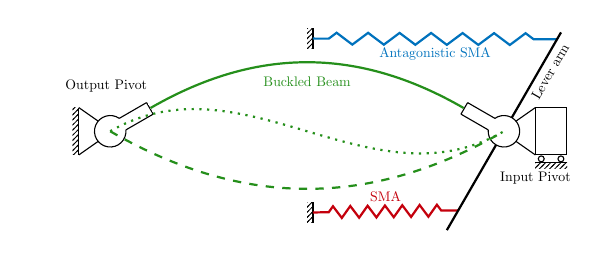
\begin{tikzpicture}[every node/.style={inner sep=0,outer sep=0}]
\tikzstyle{sma}=[thick,decorate,decoration={zigzag,pre length=2mm,post length=2mm,segment length=2.2mm, amplitude=0.75mm}]
\tikzstyle{smalong}=[thick,decorate,decoration={zigzag,pre length=2mm,post length=2mm,segment length=4mm, amplitude=0.75mm}]
\tikzstyle{ground}=[pattern=north east hatch, hatch distance=1mm, hatch thickness=0.3pt, fill,draw=none,minimum width=2mm,minimum height=0.1mm]

    % <BB>
    \node[thin, anchor=east, pivot_node, solid, black,rotate=30 ,anchor=center] (R) at (0,0) {};
    \node[thin, pivot_node, anchor=west, solid, black,rotate=150,anchor=center] (L) at (5,0) {}; % Left pivot node
    \draw[mygreen, dotted, thick] (R.center) to[in=-150, out=30] (L.center); % Middle beam
    \draw[solid, mygreen, thick](R.east) to[in=150,out=30] coordinate[pos=0.5] (topSMA) (L.east); % Main beam
    \draw[dashed, mygreen,thick](R.center) to[in=-150,out=-30] coordinate[pos=0.5] (botSMA) (L.center); % Antagonistic beam
    % <\BB>
    % <Right Pivot>
    \draw[thin] ($(R.center)+({-0.2*cos(40)},{0.2*sin(40)})$) --+($({-0.3*cos(35)},{0.3*sin(35)})$) coordinate (pivRend1);
    \draw[thin] ($(R.center)+({-0.2*cos(40)},{-0.2*sin(40)})$) --+($({-0.3*cos(35)},{-0.3*sin(35)})$) coordinate (pivRend2);
    \draw[thin] (pivRend1) -- coordinate[pos=0.5] (pivR) (pivRend2);
    \node (groundR) [ground,anchor=south,minimum width=17,minimum height=0.8mm, yshift=0, rotate=90] at (pivR.west) {};
    % <\Right Pivot>
    % <Preloading Screw>
    \draw[thin] ($(L.center)+({0.2*cos(40)},{0.2*sin(40)})$) --+($({0.3*cos(35)},{0.3*sin(35)})$) coordinate (pivLend1);
    \draw[thin] ($(L.center)+({0.2*cos(40)},{-0.2*sin(40)})$) --+($({0.3*cos(35)},{-0.3*sin(35)})$) coordinate (pivLend2);
    \draw[thin] (pivLend1) --+(0.4,0) coordinate (temp)
                (pivLend2) --+(0.4,0) coordinate[pos=0.5](pivL) -- (temp)
                (pivLend1) -- (pivLend2);
    \node (groundL) [ground,anchor=south,minimum width=11.5,minimum height=0.75mm, yshift=-1.75mm] at (pivL) {};
        \draw[thin] (groundL.north east) -- (groundL.north west); % Ground hatch
    \draw[draw,thin] ($(pivL.south)+(0.125,-0.05)$) circle (0.375mm); % Wheel
    \draw[draw,thin] ($(pivL.south)+(-0.125,-0.05)$) circle (0.375mm); % Wheel
    % <\Preloading Screw>
    % <Cold SMA>
    \node (groundTSMA) [ground,anchor=south,minimum width=7.5,minimum height=0.75mm, yshift=3mm, rotate=-90] at (topSMA) {};
        \draw[thin] (groundTSMA.north east) -- (groundTSMA.north west); % Ground hatch
    \draw[smalong, color=myblue] (groundTSMA.north) -- node[draw=none,above, yshift=-2.75mm,scale=0.5] {Antagonistic SMA} ($(L.center)+({1.35*cos(60)},{1.35*sin(60)})$);% <\Cold SMA>
    % <Hot SMA>
    \node (groundBSMA) [ground,anchor=south,minimum width=7.5,minimum height=0.75mm, yshift=-3mm, rotate=-90] at (botSMA) {};
        \draw[thin] (groundBSMA.north east) -- (groundBSMA.north west); % Ground hatch
    \draw[sma, color=myred] (groundBSMA.north) -- node[draw=none,below, yshift=2.5mm, scale=0.5] {SMA} ($(L.center)+({-1.16  *cos(60)},{-1.16    *sin(60)})$); % <\Hot SMA>
    % <Lever Arm>
    \draw[thick] ($(L.center)+({0.2*cos(60)},{0.2*sin(60)})$) --+($({1.25*cos(60)},{1.25*sin(60)})$) node[pos=0.6, below, sloped, scale=0.5, outer sep=4] {Lever arm};
    \draw[thick] ($(L.center)+({-0.2*cos(60)},{-0.2*sin(60)})$) --+($({-1.25*cos(60)},{-1.25*sin(60)})$); % <\Lever Arm>
    % <Labels>
    \node[draw=none, color=mygreen, scale=0.5, yshift=-5mm] at (topSMA) {Buckled Beam};
    \node[draw=none, color=black, scale=0.5, yshift=11.5mm, xshift=-1mm] at (R) {Output Pivot};
    \node[draw=none, color=black, scale=0.5, yshift=-1.2cm, xshift=0.8cm] at (L) {Input Pivot};
    % <\Labels>
\end{tikzpicture}
\end{document}
